\documentclass[aspectratio=169]{beamer}

%\includeonlyframes{current}

\usepackage[utf8]{inputenc}
\usepackage[american]{babel}
\usepackage{amsmath,amsthm}
\usepackage{unicode}
\usepackage{array,tabularx}
\usepackage{ifthen}
\usepackage{tikz}
\usetikzlibrary{matrix,decorations,decorations.text,calc,arrows,snakes,shapes,positioning,patterns}
\usepackage{tikzsymbols}

\usepackage{ulem}

\mode<presentation>{%
  \usetheme{ibm}
}

\newcommand{\C}{ℂ}
\newcommand{\R}{ℝ}
\newcommand{\Z}{ℤ}
\newcommand{\N}{ℕ}
\newcommand{\Q}{ℚ}
\newcommand{\F}{\mathbb{F}}
\renewcommand{\P}{\mathbb{P}}
\renewcommand{\O}{\mathcal{O}}
\newcommand{\tildO}{\mathcal{\tilde{O}}}
\newcommand{\poly}{\operatorname{poly}}
\newcommand{\polylog}{\operatorname{polylog}}
\newcommand{\End}{\operatorname{End}}
\newcommand{\Hom}{\operatorname{Hom}}
\newcommand{\Cl}{\operatorname{Cl}}
\newcommand{\GL}{\operatorname{GL}}
\newcommand{\SL}{\operatorname{SL}}
\newcommand{\cyc}[1]{{〈 #1 〉}}
\newcommand{\sm}[2]{\left(\protect\begin{smallmatrix}#1\protect\\#2\protect\end{smallmatrix}\right)}

\renewcommand{\a}{\mathfrak{a}}
\renewcommand{\b}{\mathfrak{b}}
\newcommand{\g}{\mathfrak{g}}
\newcommand{\G}{\mathcal{G}}
\newcommand{\E}{\mathcal{E}}
\DeclareMathOperator{\rank}{rank}

\title{Isogeny-based Cryptography}
\author{Luca De Feo}
\date[June 19-20, 2024, PQ-TLS summer school]{June 19-20, 2024\\
  PQ-TLS summer school}
\institute{IBM Research Zürich}

\begin{document}

\frame[plain]{\titlepage}

%%

\begin{frame}{Isogenies: What? Why?}
  \large
  \begin{itemize}
    \setlength{\itemsep}{2em}
  \item A descendant of Elliptic Curve Cryptography.
  \item A rich topic, with many cryptographic applications.
  \item A post-quantum generalization of discrete logarithm cryptography\dots
  \item \dots and much more!
  \item A field moving (too) fast!
  \end{itemize}
\end{frame}

%%

\begin{frame}{This course}
  \begin{description}
    \setlength{\itemsep}{2em}
  \item[Today:] Isogeny crypto without isogenies:
    \begin{itemize}
    \item Cryptographic group actions
    \item Something new
    \end{itemize}
  \item[Tomorrow:] The foundations
    \begin{itemize}
    \item Isogenies
    \item Endomorphism rings
    \item Complex and quaternionic multiplication
    \end{itemize}
  \item[Not covered:]
    \begin{itemize}
    \item The SIDH/SIKE attacks
    \item Higher dimensional abelian varieties
    \item Pre-quantum uses of isogenies
    \item A lot of protocols
    \end{itemize}
  \end{description}
\end{frame}

%%

\begin{frame}[plain]
  \begin{beamercolorbox}[sep=0.1px,center,wd=\paperwidth,sep=0.5\paperheight]{palette tertiary}
    \Huge\centering Cryptographic Group Actions
  \end{beamercolorbox}
\end{frame}

%%

\begin{frame}{A cyclic group}
  \Large
  \centering
  \begin{tikzpicture}
    \node at (0,0) {$G = \langle g\rangle$};
    
    \node (g) at (0:4) {$g$};
    \node (g2) at (30:4) {$g^2$};
    \node at (60:4) {$g^3$};
    \node at (-30:4) {$g^n = g^0 = 1$};
    
    \draw (5:4) arc (5:25:4) (35:4) arc (35:55:4) (-25:4) arc (-25:-5:4);
    \draw[dashed] (65:4) arc (65:325:4);
  \end{tikzpicture}
\end{frame}

%%

\begin{frame}{What's needed for key exchange?}
  \begin{columns}
    \begin{column}{0.5\textwidth}
      \centering
      \begin{tikzpicture}
        \begin{uncoverenv}<-3>
          \begin{scope}
            \def\crater{13}
            \def\jumpa{-8}
            \def\diam{2.5cm}

            \uncover<1>{
              \foreach \i in {1,...,\crater} {
                \draw[blue!20!white] (360/\crater*\i : \diam) to[bend right] (360/\crater*\i+360/\crater : \diam);
              }
            }

            \uncover<2->{
              \pgfmathparse{int(\crater/2)}
              \let\last\pgfmathresult
              \foreach \i in {1,...,\last} {
                \pgfmathparse{mod(pow(2,\i-1),\crater)}
                \let\e\pgfmathresult
                \draw[red] (360/\crater*\e : \diam) to[bend left] (360/\crater*\e*2 : \diam);
                \draw[red] (-360/\crater*\e : \diam) to[bend right] (-360/\crater*\e*2 : \diam);
              }
            }

            \uncover<3->{
              \pgfmathparse{int(\crater/2)}
              \let\last\pgfmathresult
              \foreach \i in {1,...,\last} {
                \pgfmathparse{mod(pow(6,\i-1),\crater)}
                \let\e\pgfmathresult
                \draw[blue] (360/\crater*\e : \diam) to[bend right] (360/\crater*\e*6 : \diam);
                \draw[blue] (-360/\crater*\e : \diam) to[bend left] (-360/\crater*\e*6 : \diam);
              }
            }
            
            \pgfmathparse{\crater-1}
            \let\last\pgfmathresult
            \foreach \i in {0,...,\last} {
              \draw[fill] (360/\crater*\i: \diam) circle (2pt) +(360/\crater*\i: 0.5) node{$g^{\i}$};
            }
          \end{scope}
        \end{uncoverenv}
        
        \begin{uncoverenv}<4->
          \begin{scope}
            \def\crater{12}
            \def\jumpa{5}
            \def\diam{2.5cm}

            \foreach \i in {1,...,\crater} {
              \draw[red] (360/\crater*\i : \diam) to[bend right] (360/\crater*\i+360/\crater : \diam);
              \draw[blue] (360/\crater*\i : \diam) to[bend right=10] (360/\crater*\i+\jumpa*360/\crater : \diam);
            }

            \foreach \i in {1,...,\crater} {
              \pgfmathparse{int(mod(pow(2,\i-1),\crater+1))}
              \let\e\pgfmathresult
              \draw[fill] (360/\crater*\i: \diam) circle (2pt) +(360/\crater*\i: 0.5) node{$g^{\e}$};
            }
          \end{scope}
        \end{uncoverenv}
      \end{tikzpicture}
    \end{column}
    \begin{column}{0.4\textwidth}
      The axioms of a dlog group:
      \begin{itemize}
      \item[\sout{prod:}] \sout{$g^ag^b = g^{a+b}$,}
      \item[exp:] $(g^a)^n = g^{na}$.
      \end{itemize}

      \bigskip
      The hard problem:
      \begin{itemize}
      \item[dlog:] $g^a \mapsto a$.
      \end{itemize}

      \bigskip
      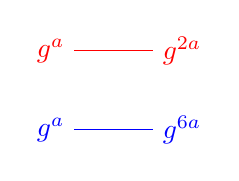
\begin{tikzpicture}
        \uncover<2->{\draw[red] (0,0) node[anchor=east]{$g^a$} -- (1,0) node[anchor=west] {$g^{2a}$};}
        \uncover<3->{\draw[blue] (0,-1) node[anchor=east]{$g^a$} -- (1,-1) node[anchor=west] {$g^{6a}$};}
      \end{tikzpicture}

      \bigskip
      \begin{uncoverenv}<5->
        Automorphism group: \emph{$(\Z/13\Z)^\times$}.
      \end{uncoverenv}
    \end{column}
  \end{columns}
\end{frame}

%%

\begin{frame}
  \begin{block}{Group action}
    \emph{$\G\circlearrowright\E$}: A (finite) set $\E$ \emph{acted
      upon} by a group $\G$ \emph{freely} and \emph{transitively}:
    \begin{align*}
      * : \G × \E &→ \E\\
      \g * E &↦ E'
    \end{align*}
    \par\begin{description}
    \item[Compatibility:] \emph{$\g' * (\g * E) = (\g'\g)*E$} for all
      $\g,\g'\in\G$ and $E\in\E$;
    \item[Identity:] \emph{$\mathfrak{e} * E = E$} if and only if
      $\mathfrak{e}\in\G$ is the identity element;
    \item[Regularity:] for all $E,E'\in\E$ there exist a \emph{unique
        $\g\in\G$} such that \emph{$\g*E'=E$}.
      \setlength{\itemsep}{2em}
    \end{description}
  \end{block}
\end{frame}

%%

\begin{frame}{Cryptographic Group Actions \small(Alamati, D., Montgomery, Patranabis 2021)}
  \begin{block}{Hard Homogeneous Space (HHS) --- Couveignes 1997 \small(eprint:2006/291)}
    \emph{$\G\circlearrowright\E$} such that $\G$ is commutative and:
    \begin{itemize}
    \item \emph{Evaluating} $E' = \g*E$ is \emph{easy};
    \item \emph{Inverting} the action is \emph{hard}.
    \end{itemize}
  \end{block}

  \begin{block}{Example}
    Let $G$ be a group of order $13$, then \emph{$(\Z/13\Z)^\times \circlearrowright G$} defined by
    \[a * g := g^a\]
    is an HHS\dots\pause
    But
    \[\alert{g^a \cdot g^b = g^{a+b}}\]
    has no interpretation as a group action!
  \end{block}
\end{frame}

%%

\begin{frame}{Key exchange from group actions}
  \begin{description}
  \item[Public parameters:] A \emph{HHS $\G\circlearrowright \E$} of
    order $N$ (large, but not necessarily prime).
  \end{description}

  \bigskip
  
  \begin{center}
    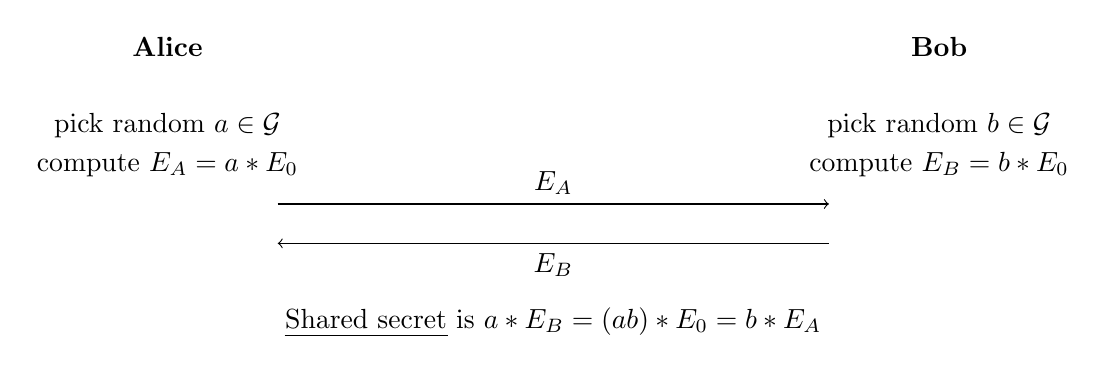
\begin{tikzpicture}[x=1.4cm]
      \node at (0,0) {\bf Alice};
      \node at (7,0) {\bf Bob};
      \node at (0,-1) {pick random \alert{$\a\in\G$}};
      \node at (0,-1.5) {compute $E_A=\a*E_0$};
      \node at (7,-1) {pick random \alert{$\b\in\G$}};
      \node at (7,-1.5) {compute $E_B=\b*E_0$};
      \draw[->]
      (1,-2) to node[auto] {$E_A$} (6,-2);
      \draw[->] (6,-2.5) to node[auto] {$E_B$} (1,-2.5);
      \node at (3.5,-3.5) {\emph{Shared secret} is \alert{$\a*E_B=(\a\b)*E_0=\b*E_A$}};
    \end{tikzpicture}
  \end{center}
\end{frame}

%%

\begin{frame}{Quantum security}

  \textbf{Fact:} Shor's algorithm \emph{does not apply} to Diffie-Hellman
  protocols from \emph{group actions}.

  \begin{block}{Subexponential attack\hfill\emph{$\exp(\sqrt{\log N\log\log N})$}}
    \begin{itemize}
    \item Reduction to the \emph{hidden shift problem} by evaluating
      the group action in \emph{quantum superposition} (subexponential
      cost);
    \item Well known reduction from the hidden shift to the
      \emph{dihedral (non-abelian) hidden subgroup problem};
    \item Kuperberg's algorithm solves the dHSP with a subexponential
      number of class group evaluations.
    \item Analyses suggest that $2^{64}$-qbit security may be achieved
      somewhere around $\log N \approx 2048$.
    \end{itemize}
  \end{block}
\end{frame}

%%

\begin{frame}{A $\Sigma$-protocol from group actions \small(Stolbunov 2008)}
  \begin{columns}
    \begin{column}{0.55\textwidth}
      Building block of Seasign and CSI-FiSh:

      \medskip
      \begin{itemize}
      \item<1-> A key pair \emph{$(\frak{s}, \frak{s}*E)$};
      \item<2-> Commit to a \emph{random element $\frak{r}*E$};
      \item<3-> Challenge with bit \emph{$b\in\{0,1\}$};
      \item<4-> Respond with \emph{$\frak{c} = \frak{r}/\frak{s}^b$};
      \item<5-> Verify that \emph{$\frak{c}*\frak{s^b}*E = \frak{r}*E$}.
      \end{itemize}

      \begin{block}{Zero-knowledge}<6->
        \centering
        Does not leak if:\\
        \alert{$\frak{c}$ is uniformly distributed} and independent from $\frak{s}$.
      \end{block}

    \end{column}  
    \begin{column}{0.40\textwidth}
      \centering
      \begin{tikzpicture}
        \node (g) at (0,0) {$E$};
        \node (gs) at (3,0) {$E_s$};
        \path[->] (g) edge node[auto]{$\frak{s}$} (gs);
        \uncover<2->{
          \node (gr) at (1.5,-3) {$E_r$};
          \path[->] (g) edge node[auto,swap]{$\frak{r}$} (gr);
        }
        \uncover<4->{
          \path[dashed,->] (gs) edge node[auto]{$\frak{r}/\frak{s}$} (gr);
        }
      \end{tikzpicture}
    \end{column}  
  \end{columns}
\end{frame}

%%

\begin{frame}{How isogenies may fail the axioms}
  \begin{block}{\alt<2->{\sout{Hard Homogeneous Space (HHS)}}{Hard
        Homogeneous Space (HHS)} \uncover<2->{Restricted Effective Group Action (REGA)}}
    \emph{$\G\circlearrowright\E$} such that $\G$ is commutative and:
    \begin{itemize}
    \item \emph{Inverting} the action is \emph{hard}.
    \item \alt<2->{\sout{\emph{Evaluating} $E' = \g*E$ is \emph{easy};}}{\emph{Evaluating} $E' = \g*E$ is \emph{easy};}
    \item<2-> There is a small list of elements
      \emph{$(\g_1, \ldots, \g_n)$} such that evaluating $E' = \g_i*E$
      is easy.
    \end{itemize}
  \end{block}
  
  \begin{uncoverenv}<3->
    Assume that $(\g_1, \ldots, g_n)$ generates $\G$:
    \begin{align*}
      \Z^n &\twoheadrightarrow \G\\
      (a_1,\ldots,a_n)&\mapsto \g_1^{a_1}\cdots g_n^{a_n}
    \end{align*}
    Extend $\G\circlearrowright\E$ to an action
    \emph{$\Z^n\circlearrowright\E$} (not free):
    \[(a_1, \ldots, a_n) * E \quad:=\quad \g_1^{a_1} * \cdots * \g_n^{a_n} * E.\]
  \end{uncoverenv}
\end{frame}

%%

\begin{frame}{Crypto from REGAs}
  \[(a_1, \ldots, a_n) * E \quad:=\quad \g_1^{a_1} * \cdots * \g_n^{a_n} * E.\]

  \begin{itemize}
  \item Evaluation efficient for vectors in $\Z^n$ of \emph{small norm};
  \item Key exchange works unmodified;
  \item<2-> Signature breaks down:
    \begin{columns}
      \begin{column}{0.40\textwidth}
        \begin{itemize}
        \item A key pair \emph{$(\vec{s}, \vec{s}*E)$};
        \item Commit to a \emph{random element $\vec{r}*E$};
        \item Challenge with bit \emph{$b\in\{0,1\}$};
        \item \alert{Respond with $\vec{c} = \vec{r} - b\cdot\vec{s}$};
        \item Verify that \emph{$\vec{c}*(b\cdot\vec{s})*E = \vec{r}*E$}.
        \end{itemize}
        Distribution of \alert{$\vec{r}-\vec{s}$} depends on \alert{$\vec{s}$}.
      \end{column}
      \begin{column}{0.40\textwidth}
        \centering
        \begin{tikzpicture}
          \node (g) at (0,0) {$E$};
          \node (gs) at (3,0) {$E_s$};
          \path[->] (g) edge node[auto]{$\vec{s}$} (gs);
          \node (gr) at (1.5,-3) {$E_r$};
          \path[->] (g) edge node[auto,swap]{$\vec{r}$} (gr);
          \path[dashed,->] (gs) edge node[auto]{$\vec{r} - \vec{s}$} (gr);
        \end{tikzpicture}
      \end{column}
    \end{columns}

    \medskip
    Fix: \emph{rejection sampling}. Very expensive!
  \end{itemize}
\end{frame}

%%

\begin{frame}{How to transform a REGA in an Effective Group Action again}
  \begin{align*}
    \Z^n &\twoheadrightarrow \G\\
    (a_1,\ldots,a_n)&\mapsto \g_1^{a_1}\cdots g_n^{a_n}
  \end{align*}
  The kernel is an integral lattice $\Lambda$, and
  \emph{$\G \simeq Z^n/\Lambda$}.

  \begin{enumerate}
  \item Compute the kernel $\Lambda$
    \begin{itemize}
    \item In \emph{subexponential} $L(1/2)$ time for isogenies, or
    \item In \emph{quantum polynomial time} for any group;
    \end{itemize}
  \item Compute generators of $\Z^n/\Lambda$;
  \item Use lattice reduction to convert elements of $\Z^n/\Lambda$ to
    vectors of \emph{small norm}.
  \end{enumerate}

  \pause
  \begin{block}{Applications \small(Beullens, Kleinjung, Vercauteren 2019; D., Meyer 2020)}
    \begin{itemize}
    \item \emph{CSI-FiSh}: reasonably short and not too slow signatures.
    \item If \emph{$\G=\langle\g\rangle$} is cyclic of order
      \emph{$N$}, explicit action \emph{$\Z/N\Z\circlearrowright\E$}:
      $\qquad a * E := \g^a * E$\\
      $\to$ \emph{threshold signatures} via Shamir secret sharing.
    \end{itemize}
  \end{block}
\end{frame}

%%

\begin{frame}[plain]
  \begin{beamercolorbox}[sep=0.1px,center,wd=\paperwidth,sep=0.5\paperheight]{palette tertiary}
    \Huge\centering Something new
  \end{beamercolorbox}
\end{frame}

%%

\begin{frame}{Objects \uncover<2>{and Morphisms}}
  \centering
  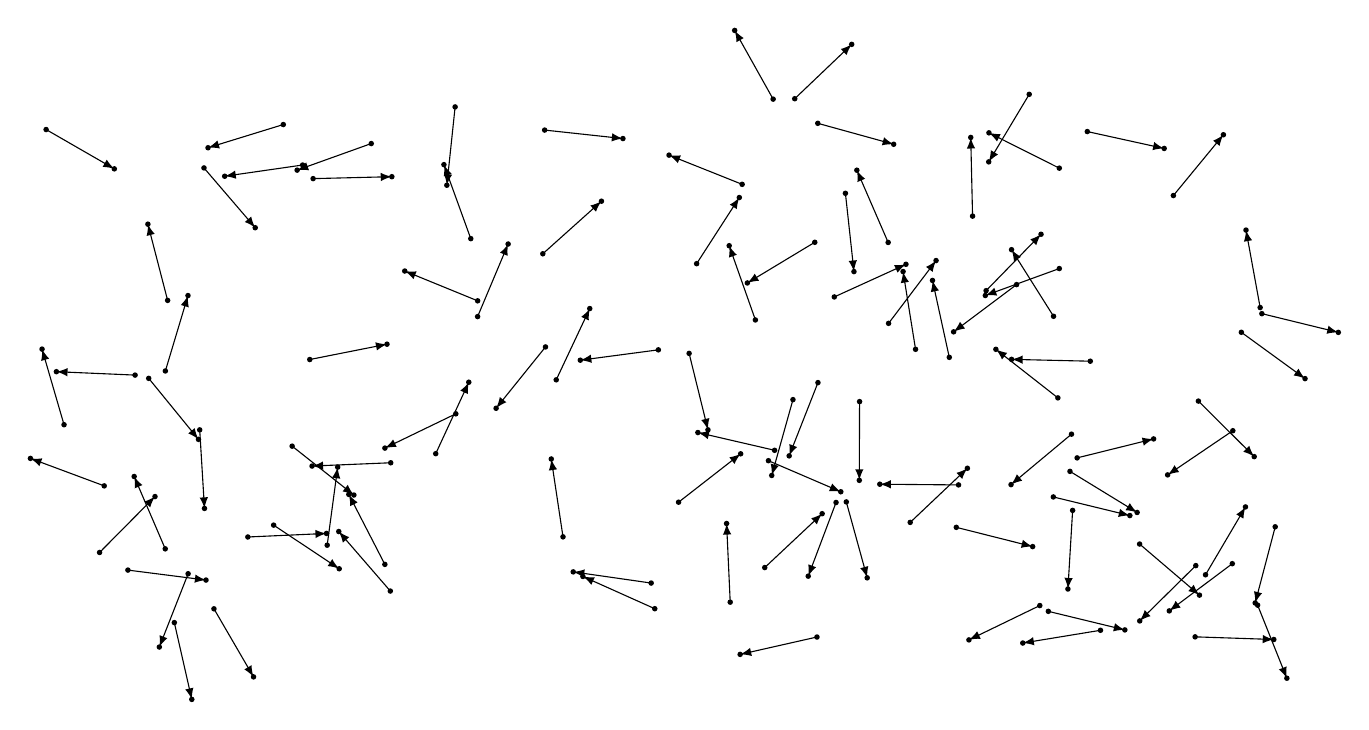
\begin{tikzpicture}
    \pgfmathsetseed{12345}
    \foreach \i in {1,...,100} {
      \pgfmathparse{16*random()}
      \let\x\pgfmathresult
      \pgfmathparse{7*random()}
      \let\y\pgfmathresult
      \pgfmathparse{360*random()}
      \let\ang\pgfmathresult
      \pgfmathparse{7*random()}
      \fill (\x,\y) circle (1pt) +(\ang:1) circle (1pt);
      \uncover<2>{\draw[-latex] (\x,\y) to +(\ang:1);}
    }
  \end{tikzpicture}  
\end{frame}

%%

\begin{frame}{More than graphs\dots}
  \begin{itemize}
  \item A finite set of \emph{objects} $\E$,
  \item For each pair $A,B\in\E$ a set of \emph{morphisms} $\Hom(A,B)$
  \end{itemize}

  \vfill
  
  \centering
  \begin{tikzpicture}
    \node (E1) at (0,0) {$B$};
    \node (E) at (6,0) {$A$};

    \draw[-latex] (E) edge node[above] {$φ$} (E1);
    \node at (3,-1.5) {$φ ∈ \Hom(A,B)$};

    \uncover<2->{
      \draw[-latex] (E) edge[loop,out=45,in=-45,looseness=10] node[right] {$ω$} (E);
      \node at (8,-1.5) {$ω ∈ \Hom(A,A)$};
    }
  \end{tikzpicture}
\end{frame}

%%

\begin{frame}{Transitively closed}
  \centering
  \begin{tikzpicture}
    \node (A) at (0,0) {$A$};
    \node (B) at (-6,0) {$B$};
    \node (C) at (-12,0) {$C$};

    \draw[-latex]
    (A) edge node[above] {$φ$} (B)
    (B) edge node[above] {$ψ$} (C);

    \uncover<2->{
      \draw[-latex]
      (A) edge[bend left] node[below] {$ψ∘φ$} (C);
    }
  \end{tikzpicture}
\end{frame}

%%

\begin{frame}{Identity morphisms}
  \centering
  \begin{tikzpicture}
    \node (A) at (0,0) {$A$};
    \node (B) at (-6,0) {$B$};
    \draw[-latex]
    (A) edge node[above] {$φ$} (B)
    (A) edge[loop,out=45,in=-45,looseness=10] node[right] {$1_A$} (A)
    (B) edge[loop,out=135,in=225,looseness=10] node[left] {$1_B$} (B);
    \node at (-3,-1.5) {$1_B∘φ \;=\; φ \;=\; φ∘1_A$};
  \end{tikzpicture}
\end{frame}

%% 

\begin{frame}{Ab-categories}
  \large
  \begin{itemize}
    \setlength{\itemsep}{2em}
  \item $\Hom(A,B)$ is a group
  \item Distributivity:
    \begin{align*}
      φ∘(ψ+χ) &= (φ∘ψ)+(φ∘χ)\\[2em]
      (ψ+χ)∘φ &= (ψ∘φ)+(χ∘φ)\\
    \end{align*}
  \item It follows that \emph{$\End(A) := \Hom(A,A)$} is a ring.
  \end{itemize}
\end{frame}

%%

\begin{frame}{Computational properties}
  \large
  \begin{itemize}
    \setlength{\itemsep}{2em}
  \item Every object and every morphism has a unique representation as
    a string;
  \item The representation of a morphism $\phi:A\to B$ identifies $A$
    and $B$;
  \item There exists efficient algorithms to verify that a string
    represents an object/morphism;
  \item There exists an \emph{origin object} $O \in \E$ whose
    representation is known;
  \item \dots
  \end{itemize}
\end{frame}

%%

\begin{frame}{\textit{Walking}}
  \large
  Efficient algorithm for:
  
  \bigskip
  \begin{description}
  \item[Input:] Object $A$
  \item[Output:]
    \begin{itemize}
    \item Uniformly random object $B$,
    \item Random morphism $\phi:A\to B$.
    \end{itemize}
  \end{description}
\end{frame}

%%

\begin{frame}{\textit{Triangulating}}
  \centering
  \begin{tikzpicture}
    \node (O) at (0,0) {$O$};
    \node (A) at (2,-4) {$A$};
    \node (B) at (-2,-4) {$B$};
    \draw[-latex] (O) edge (A) edge (B);
    \node at (0,-5) {\emph{Input}};
    \uncover<2->{
      \node (AA) at (10,-4) {$A$};
      \node (BB) at (6,-4) {$B$};
      \draw[-latex] (AA) edge node[above] {random} (BB);
      \node at (8,-5) {\emph{Output}};
    }
  \end{tikzpicture}
\end{frame}

%%

\begin{frame}{Assumption 1}
  Given $A, B$ hard to find $\phi: A \to B$

  \vfill
  
  \centering
  \begin{tikzpicture}
    \node (A) at (0,0) {$A$};
    \node (B) at (-6,0) {$B$};
    \draw[-latex,dashed] (A) edge (B);
  \end{tikzpicture}
\end{frame}

%%

\begin{frame}{Assumption 2}
  These two distributions are indistinguishable:

  \vfill

  \begin{columns}
    \begin{column}{0.5\textwidth}
      \begin{itemize}
      \item Given $A$,
      \item \emph{\textit{Walk} $\phi : A \to B$,}
      \end{itemize}
    \end{column}
    \begin{column}{0.5\textwidth}
      \begin{itemize}
      \item Given $O \to A$,
      \item Sample random $O \to B$,
      \item \emph{\textit{Triangulate} $\phi : A \to B$} 
      \end{itemize}
    \end{column}
  \end{columns}
\end{frame}

%%

\begin{frame}[plain]
  \begin{beamercolorbox}[sep=0.1px,center,wd=\paperwidth,sep=0.5\paperheight]{palette tertiary}
    \Huge\centering Isogenies
  \end{beamercolorbox}
\end{frame}

%%

\begin{frame}{Elliptic curves}
  \begin{columns}
    \begin{column}{0.4\textwidth}
      {\Large
      \[y^2 = x^3 + ax + b\]
      }
      \begin{block}{Bezout's theorem}
        Every line cuts $E$ in exactly three points (counted with
        multiplicity).
      \end{block}

      Define a \emph{group law} such that any three colinear points
      add up to zero.
    \end{column}
    \begin{column}{0.6\textwidth}
      \begin{center}
        \begin{tikzpicture}[domain=-2.4566:4,samples=100,yscale=1/2]
          \draw plot (\x,{sqrt(\x*\x*\x-4*\x+5)});
          \draw plot (\x,{-sqrt(\x*\x*\x-4*\x+5)});

          \draw[thin,gray,-latex] (0,-7) -- (0,7);
          \draw[thin,gray,-latex] (-3,0) -- (4,0);
          \draw (-3,1) -- (4,8/3+3);
          \begin{scope}[every node/.style={draw,circle,inner sep=1pt,fill},cm={1,2/3,0,0,(0,3)}]
            \node at (-2.287980,0) {};
            \node at (-0.535051,0) {};
            \node at (3.267475,0) {};
          \end{scope}
          \begin{scope}[every node/.style={yshift=0.3cm},cm={1,2/3,0,0,(0,3)}]
            \node at (-2.287980,0) {$P$};
            \node at (-0.535051,0) {$Q$};
            \node at (3.267475,0) {$R$};
          \end{scope}

          \draw[dashed] (3.267475,3.267475*2/3+3) -- (3.267475,-3.267475*2/3-3) 
          node[draw,circle,inner sep=1pt,fill] {}
          node[xshift=-0.1cm,anchor=east] {$P+Q$};
        \end{tikzpicture}
      \end{center}
    \end{column}
  \end{columns}
\end{frame}

%% 

\begin{frame}
  \Large
  \begin{description}
    \setlength{\itemsep}{4em}
  \item[Isogenies =] finite-kernel algebraic group morphisms: \emph{$E \to E/K$}
  \item[Endomorphisms =] isogenies \emph{$E \to E$}
  \end{description}
\end{frame}

%%

\begin{frame}{Isogenies: an example over $\F_{11}$}
  \centering
  \begin{tikzpicture}[scale=0.4]
    \begin{scope}
      \node[anchor=center] at (0,7) {$E \;:\; y^2 = x^3 + x$};

      \uncover<-1>{
        \draw[thin,gray] (0,-6) -- (0,6);
        \draw[thin,gray] (-6,0) -- (6,0);
      }

      \foreach \x/\y in {0/0,5/3,-4/3,-3/5,-2/1,-1/3} {
        \draw[blue,fill] (\x,\y) circle (0.2) node(E_\x_\y){}
        (\x,-\y) circle (0.2) node(E_\x_-\y){};
      }

      \uncover<2->{\draw[red,fill] (0,0) circle (0.3);}
    \end{scope}

    \draw[black!10!white,thick] (10,-7) -- +(0,14);
    
    \begin{scope}[shift={(20,0)}]
      \node at (0,7) {$E' \;:\; y^2 = x^3 - 4x$};

      \uncover<-1>{
        \draw[thin,gray] (0,-6) -- (0,6);
        \draw[thin,gray] (-6,0) -- (6,0);
      }

      \foreach \x/\y in {0/0,2/0,3/2,4/2,6/4,-2/0,-1/5} {
        \draw[color=blue,fill] (\x,\y) circle (0.2) node(F_\x_\y){}
        (\x,-\y) circle (0.2) node(F_\x_-\y){};
      }
    \end{scope}

    \begin{scope}[color=red,-latex,dashed]
      \begin{uncoverenv}<2->
        \path
        (E_5_3) edge (F_3_2)
        (E_-4_3) edge (F_4_-2)
        (E_-3_5) edge (F_4_2)
        (E_-2_1) edge (F_3_-2)
        (E_-1_3) edge (F_-2_0);
      \end{uncoverenv}
      \begin{uncoverenv}<2->
        \path
        (E_5_-3) edge (F_3_-2)
        (E_-4_-3) edge (F_4_2)
        (E_-3_-5) edge (F_4_-2)
        (E_-2_-1) edge (F_3_2)
        (E_-1_-3) edge (F_-2_0);
      \end{uncoverenv}
    \end{scope}
  \end{tikzpicture}
  
  \begin{columns}
    \begin{column}{0.5\textwidth}
      \[\phi(x,y) = \left(\frac{x^2 + 1}{x},\quad y\frac{x^2-1}{x^2}\right)\]
    \end{column}
    \begin{column}{0.5\textwidth}
      \begin{itemize}
      \item<2-> Kernel generator in \alert{red}.
      \item<2-> This is a degree $2$ map.
      \item<2-> Analogous to $x\mapsto x^2$ in $\F_q^*$.
      \end{itemize}
    \end{column}
  \end{columns}
\end{frame}

%%

\begin{frame}{Some endomorphisms}
  \Large
  \begin{description}
    \setlength{\itemsep}{3em}
  \item[Scalar multiplication:] $[N] : E \to E$
  \item[Frobenius:] $(x,y) \mapsto (x^p, y^p)$ \hfill(on curves over $\F_p$)
  \item[Automorphisms:] $(x,y) \mapsto (-x, iy)$ \hfill(on curve $y^2 = x^3 + x$)
  \end{description}
\end{frame}

%%

\begin{frame}{Transitively closed}
  \centering
  \begin{tikzpicture}
    \node (A) at (0,0) {$A$};
    \node (B) at (-6,0) {$B$};
    \node (C) at (-12,0) {$C$};

    \draw[-latex]
    (A) edge node[above] {$φ$} (B)
    (B) edge node[above] {$ψ$} (C);

    \draw[-latex]
    (A) edge[bend left] node[below] {$ψ∘φ$} (C);
  \end{tikzpicture}
\end{frame}

%%

\begin{frame}{Identity morphisms}
  \centering
  \begin{tikzpicture}
    \node (A) at (0,0) {$A$};
    \node (B) at (-6,0) {$B$};
    \draw[-latex]
    (A) edge node[above] {$φ$} (B)
    (A) edge[loop,out=45,in=-45,looseness=10] node[right] {$1_A$} (A)
    (B) edge[loop,out=135,in=225,looseness=10] node[left] {$1_B$} (B);
    \node at (-3,-1.5) {$1_B∘φ \;=\; φ \;=\; φ∘1_A$};
  \end{tikzpicture}
\end{frame}

%% 

\begin{frame}{Ab-categories}
  \large
  \begin{itemize}
    \setlength{\itemsep}{2em}
  \item $\Hom(A,B)$ is a group
  \item Distributivity:
    \begin{align*}
      φ∘(ψ+χ) &= (φ∘ψ)+(φ∘χ)\\[2em]
      (ψ+χ)∘φ &= (ψ∘φ)+(χ∘φ)\\
    \end{align*}
  \item It follows that \emph{$\End(A) := \Hom(A,A)$} is a ring.
  \end{itemize}
\end{frame}

%%

\begin{frame}[plain]
  \begin{beamercolorbox}[sep=0.1px,center,wd=\paperwidth,sep=0.5\paperheight]{palette tertiary}
    \Huge\centering The Endomorphism Ring
  \end{beamercolorbox}
\end{frame}

%%

\begin{frame}{$N$-torsion}
  \large
  \begin{columns}
    \begin{column}{0.45\textwidth}
      Over an algebraically closed field, for any $N$ coprime to the characteristic:
      \[\emph{E[N] \simeq ℤ/Nℤ \times ℤ/Nℤ}\]
    \end{column}
    \begin{column}{0.45\textwidth}
      \centering
      \begin{tikzpicture}
        \draw[dashed,gray] (0,-.5) to (0,5) (-.5,0) to (5,0);
        \foreach \i in {0,...,4} {
          \foreach \j in {0,...,4} {
            \fill (\i,\j) circle(2pt);
          }
        }
        {
          \small
          \draw[red] (0,1) node[left]{$P$} (1,0) node[below]{$Q$};
        }
      \end{tikzpicture}
    \end{column}
  \end{columns}
\end{frame}

%%

\begin{frame}{Endomorphisms = $2 \times 2$ matrices}
  Fix any basis \emph{$〈P,Q〉$} of \emph{$E[N]$}

  \begin{align*}
    \omega : E[N] &→ E[N]\\
    \begin{pmatrix}
      x\\y
    \end{pmatrix}
                  &↦
                    \begin{pmatrix}
                      a&b\\c&d
                    \end{pmatrix}
                              \begin{pmatrix}
                                x\\y
                              \end{pmatrix}
    \mod N
  \end{align*}
  
  \begin{block}{Tate's isogeny theorem}
    When $E$ is supersingular:
    
    \[\emph{\End(E)/N\End(E) ≃ \mathcal{M}_{2\times 2}(ℤ/Nℤ)}\]

    When $E$ is ordinary:

    \[\emph{\End(E)/N\End(E) ≃ \{\text{Diagonal matrices}\} ⊂ \mathcal{M}_{2\times 2}(ℤ/Nℤ)}\]
  \end{block}
\end{frame}

%%

\begin{frame}{Endomorphisms = imaginary quadratic integers}
  \large
  Endomorphisms form a ring:
  \[ω ∘ (φ + ψ) \quad=\quad ω∘φ + ω∘ψ\]

  \bigskip
  Every endomorphism satisfies a quadratic equation
  \[ω^2 - tω + n = 0\]
  with $t,n ∈ ℤ$ and $t^2 - 4n ≤ 0$.
\end{frame}

%% 

\begin{frame}{Endomorphism rings = Ideal lattices}
  \Large $\End(E)$ is a free $ℤ$-module of rank \textcolor{blue}{1},
  \textcolor{purple}{2} or \textcolor{red}{4}. As a ring:

  \bigskip
  \begin{enumerate}
    \setlength{\itemsep}{1em}
  \item[\color{blue}1)] $\End(E) ≃ ℤ$;
  \item[\color{purple}2)] $\End(E)$ is isomorphic to an
    order\footnote[1]{order = subring of maximal rank} of a quadratic
    imaginary field;
  \item[\color{red}4)] $\End(E)$ is isomorphic to a maximal
    order\footnotemark[1] of the quaternion algebra ramified at $p$
    and $∞$.
  \end{enumerate}
\end{frame}

%% 

\begin{frame}{\color{purple}Quadratic imaginary number fields}
  \large
  \[ℚ(\sqrt{-D}) \qquad\text{with}\qquad D>0\]

  \bigskip
  \begin{itemize}
    \setlength{\itemsep}{1em}
  \item \textcolor{purple}{$2$-dimensional} $ℚ$-vector space,
  \item Unique maximal order $\quad=\quad$ ring of integers.
  \end{itemize}
\end{frame}

%%

\begin{frame}{\color{red}Quaternion algebras}
  (Assume $p=-1 \bmod 4$) The quaternion algebra \emph{$B_{p,∞}$} is:
  \begin{itemize}
  \item A \textcolor{red}{$4$-dimensional} $ℚ$-vector space with basis
    \emph{$(1,i,j,k)$}.
  \item A non-commutative \emph{division algebra}%
    \footnote{All elements have inverses.} %
    $B_{p,∞} = ℚ〈i,j〉$ with the relations:
    \[i^2 = -1, \quad j^2 = -p, \quad ij = -ji = k.\]
  \end{itemize}

  \begin{block}{Properties}
    \begin{itemize}
    \item All elements of $B_{p,∞}$ are \emph{quadratic algebraic
        numbers}.
    \item $B_{p,∞}⊗ℚ_ℓ≃\mathcal{M}_{2×2}(ℚ_ℓ)$ for all $ℓ≠p$.\\
    \item $B_{p,∞}⊗ℝ$ is isomorphic to Hamilton's quaternions.
    \item $B_{p,∞}⊗ℚ_p$ is a division algebra.
    \end{itemize}
  \end{block}
\end{frame}

%%

\begin{frame}{An example}
  The curve of $j$-invariant \emph{$1728$}
  \[E: y^2 = x^3 + x\]
  is supersingular over $\F_p$ iff $p=-1\mod 4$.

  \begin{block}{Endomorphisms}
    \emph{$\End(E) ⊂ ℚ〈ι,π〉$}, with:
    \begin{itemize}
    \item $π$ the Frobenius endomorphism, s.t. \emph{$π^2=-p$};
    \item $ι$ the map
      \[ι(x,y) = (-x,iy),\]
      where \emph{$i∈\F_{p^2}$} is a 4-th root of unity.
      Clearly, \emph{$ι^2=-1$}.
    \end{itemize}
    And \emph{$ιπ=-πι$}.
  \end{block}
\end{frame}

%%

\begin{frame}{Isogenies = Ideals}
  \large\centering
  \begin{tikzpicture}
    \node (E1) at (0,0) {$E'$};
    \node (E) at (6,0) {$E$};

    \draw[-latex] (E) edge node[above] {$φ$} (E1);
    \uncover<1>{
      \node at (3,-3) {$φ ∈ \Hom(E,E')$};
    }

    \uncover<2>{
      \draw[-latex] (E) edge[loop,out=45,in=-45,looseness=10] node[right] {$ω$} (E);
      \node at (3,-3) {$φ∘ω ∈ \Hom(E,E')$};
    }
    
    \uncover<3>{
      \draw[-latex] (E1) edge[loop,out=135,in=225,looseness=10] node[left] {$ω'$} (E1);
      \node at (3,-3) {$ω'∘φ ∈ \Hom(E,E')$};
    }
  \end{tikzpicture}
\end{frame}

%%

\begin{frame}{Isogenies = Ideals}
  \large
  Let \emph{$\phi : E → E/K$} be an isogeny
  \bigskip
  \[I_\phi = \{ ω ∈ \End(E) \;\mid\; ω(K) = 0 \}\]

  \bigskip
  
  Let \emph{$I ⊂ \End(E)$} be an \textit{invertible} ideal
  \begin{align*}
    E[I] &= \bigcap_{ω∈I} \ker ω,\\
    \phi_I &: E → E/E[I]
  \end{align*}

  \bigskip

  \emph{Deuring:} this is a 1-to-1 correspondence.
\end{frame}

%%

\begin{frame}{The Deuring correspondences}
  \centering\large
  \setlength{\tabcolsep}{2em}
  \renewcommand{\arraystretch}{1.8}
  \begin{tabular}{r l}
    \emph{Ellitpic curves} & \emph{Number fields / Quaternion algebras}\\
    \hline
    Endomorphisms & Algebraic integers\\
    Endomorphism ring & (Maximal) order\\
    Isogeny & Ideal\\
    Isogeny degree & Ideal norm\\
    Isogeny composition & Ideal multiplication\\
    \color{gray}Isogenies \raisebox{-0.8em}{\tikz{\node (E) at (0,0) {$\bullet$}; \node (E1) at (2,0) {$\bullet$}; \draw[->] (E) edge[bend left] (E1) edge[bend right] (E1);}} & \color{gray}Ideal classes\\
    \color{gray}Dual isogeny & \color{gray}Conjugate ideal\\
  \end{tabular}
\end{frame}

%%

\begin{frame}{Two computational worlds}
  \centering
  \setlength{\tabcolsep}{2em}
  \renewcommand{\arraystretch}{1.5}
  \begin{tabular}{p{0.3\textwidth} c c}
    & \emph{Ordinary / CSIDH} & \emph{Supersingular}\\
    \hline
    $\rank\Hom(E,E')$ & 2 & 4\\
    Endomorphism algebra & number field & quaternion algebra\\
    Maximal orders & one & many \\
    Ideal class\dots & \dots group & \dots set\\
    Find isogeny $E → E'$ & \alert{hard} & \alert{hard}\\
    Convert isogenies $\leftrightarrow$ ideals & easy\footnotemark[1] & easy\footnote[1]{When $\End(E)$ is known}\\
    Compute $\End(E)$ & easy & \alert{hard}\\
  \end{tabular}
\end{frame}

%%

\begin{frame}[plain]
  \begin{beamercolorbox}[sep=0.1px,center,wd=\paperwidth,sep=0.5\paperheight]{palette tertiary}
    \Huge\centering Quaternionic Multiplication
  \end{beamercolorbox}
\end{frame}

%%

\begin{frame}{The Deuring correspondence (for supersingular curves)}
  \begin{block}{An equivalence of categories (roughly)}
    \centering
    \begin{tikzpicture}
      \node (O) at (0,0) {$\O$};
      \node (O1) at (6,0) {$\O'$};
      \node (E) at (0,-1) {$E$};
      \node (E1) at (6,-1) {$E'$};
      
      \begin{scope}[gray,anchor=north]
        \node (Oc) at (-2,1) {left order};
        \node at (-2, 1.5) {$\{ω\in B_{p,\infty}\;|\; ωI=I\}$};
        \node (O1c) at (8,1) {right order};
        \node at (8,1.5) {$\{ω\in B_{p,\infty}\;|\; Iω=I\}$};
        \node (ac) at (3,1.5) {connecting ideal};
        
        \node (Ec) at (-2,-2) {supersingular curve};
        \node (E1c) at (8,-2) {supersingular curve};
        \node (phic) at (3,-2) {isogeny};
      \end{scope}
      
      \draw[->] (O) edge node[auto] (a) {$I$} (O1)
      (E) edge node[auto,swap] (phi) {$\phi_I$} (E1);
      \draw[dashed,->] (Oc) edge (O) (O1c) edge (O1) (ac) edge (a)
      (Ec) edge (E) (E1c) edge (E1) (phic) edge (phi);
    \end{tikzpicture}
  \end{block}
\end{frame}

%%

\begin{frame}{The effective Deuring correspondence}
  \centering\large
  \setlength{\tabcolsep}{2em}
  \renewcommand{\arraystretch}{1.8}
  \begin{tabular}{c c c}
    Input & Output \\
    \hline
    random $E$ & $\End(E)$ & \alert{hard}\\
    random $E$ & $ω ∈ \End(E)$ & \alert{hard}\\
    random $E$ & $\phi : E_0\to E$ & \alert{hard}\\
    \hline
    $\End(E)$ & $E$ & easy\\
    $\End(E)$, $\End(E')$ & connecting ideal & easy\\
    \hline
    $I ⊂ \End(E)$ & $\phi_I : E → E'$ & easy\\
    $\End(E)$,\;\; $\phi: E → E'$ & $I_\phi ⊂ \End(E)$,\;\; $\End(E')$ & easy
  \end{tabular}
\end{frame}

%%

\begin{frame}{\textit{Walking}}
  \large
  Efficient algorithm for:
  
  \bigskip
  \begin{description}
  \item[Input:] Object $A$
  \item[Output:]
    \begin{itemize}
    \item Uniformly random object $B$,
    \item Random morphism $\phi:A\to B$.
    \end{itemize}
  \end{description}
\end{frame}

%%

\begin{frame}{\textit{Triangulating}}
  \centering
  \begin{tikzpicture}
    \node (O) at (0,0) {$O$};
    \node (A) at (2,-4) {$A$};
    \node (B) at (-2,-4) {$B$};
    \draw[-latex] (O) edge (A) edge (B);
    \node at (0,-5) {\emph{Input}};

    \node (AA) at (10,-4) {$A$};
    \node (BB) at (6,-4) {$B$};
    \draw[-latex] (AA) edge node[above] {random} (BB);
    \node at (8,-5) {\emph{Output}};
  \end{tikzpicture}
\end{frame}

%%

\begin{frame}{Assumption 1}
  Given $A, B$ hard to find $\phi: A \to B$

  \vfill
  
  \centering
  \begin{tikzpicture}
    \node (A) at (0,0) {$A$};
    \node (B) at (-6,0) {$B$};
    \draw[-latex,dashed] (A) edge (B);
  \end{tikzpicture}
\end{frame}

%%

\begin{frame}{Assumption 2}
  These two distributions are indistinguishable:

  \vfill

  \begin{columns}
    \begin{column}{0.5\textwidth}
      \begin{itemize}
      \item Given $A$,
      \item \emph{\textit{Walk} $\phi : A \to B$,}
      \end{itemize}
    \end{column}
    \begin{column}{0.5\textwidth}
      \begin{itemize}
      \item Given $O \to A$,
      \item Sample random $O \to B$,
      \item \emph{\textit{Triangulate} $\phi : A \to B$} 
      \end{itemize}
    \end{column}
  \end{columns}
\end{frame}

%%

\begin{frame}{SQIsign}
  \large
  \centering
  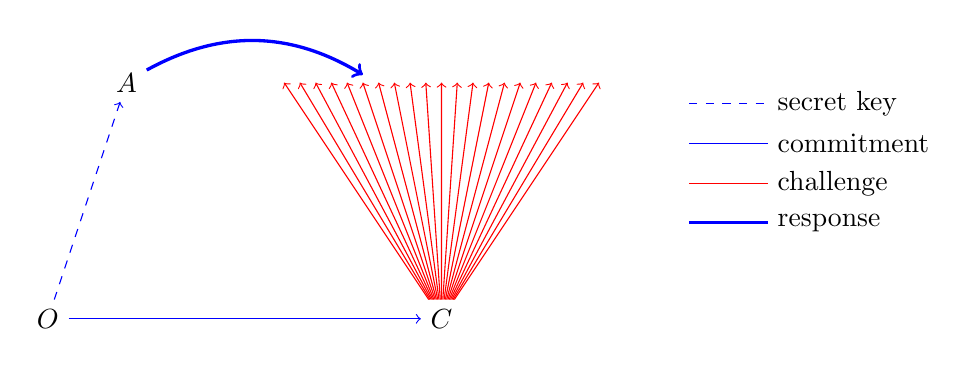
\begin{tikzpicture}
    \node (E0) at (1,3) {$A$};
    \node (EA) at (0,0) {$O$};
    \draw [blue,dashed,<-] (E0) edge (EA);

    \uncover<2->{
      \node (Ec) at (5,0) {$C$};
      \draw [blue] [->] (EA) to (Ec);
    }

    \uncover<3->{
      \foreach \x in {3,3.2,...,7} {
        \draw [red,->] (Ec) -- (\x,3);
      }
    }
    
    \uncover<4->{
      \draw [blue,very thick,->] (E0) to[bend left] (4,3.1);
    }
    
    \matrix [right] at (8,2) {
      \draw[dashed] (0,0) edge[blue] (1,0) (1,0) node {secret key};\\
      \uncover<2->{\draw (0,0) edge[blue] (1,0) (1,0) node {commitment};}\\
      \uncover<3->{\draw (0,0) edge[red] (1,0) (1,0) node {challenge};}\\
      \uncover<4->{\draw (0,0) edge[blue,very thick] (1,0) (1,0) node {response};}\\
    };
  \end{tikzpicture}
\end{frame}

%%

\begin{frame}{SQIsign}
  \begin{center}
    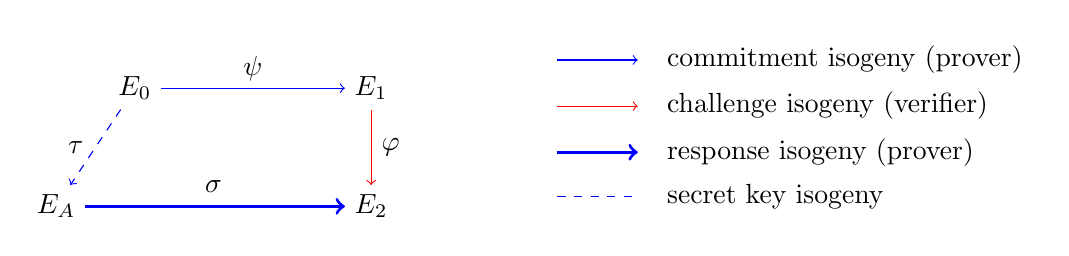
\begin{tikzpicture}
      \node (E0) at (1,2.5) {$E_0$};
        \node (E1) at (4,2.5) {$E_1$};
        \node (B) at (2.5,2.75) {$\psi$};
        \draw [blue] [->] (E0) to (E1);
        \node (E2) at (4,1) {$E_2$};
        \node (A) at (4.25,1.75) {$\varphi$};
        \draw [red] [->] (E1) to (E2);
      \node (EA) at (0,1) {$E_A$};
      \node (A) at (0.25,1.75) {$\tau$};
      \draw [blue,dashed] [->] (E0) to (EA);

        \node (B) at (2,1.25) {$\sigma$};
        \draw [blue,very thick] [->] (EA) -- (E2);

      \matrix [right] at (6,2) {
        \node[] (l1) {}; \node (l2) [right of = l1, node distance=0.5in,label=right: commitment isogeny (prover)] {}; \draw [blue] [->] (l1) -- (l2); \\
        \node[] (l3) {}; \node (l4) [right of = l3, node distance=0.5in,label=right:challenge isogeny (verifier)] {}; \draw [red] [->] (l3) -- (l4); \\
        \node[] (l1) {}; \node (l2) [right of = l1, node distance=0.5in,label=right: response isogeny (prover)] {}; \draw [blue,very thick] [->] (l1) -- (l2); \\
        \node[] (l1) {}; \node (l2) [right of = l1, node distance=0.5in,label=right: secret key isogeny] {}; \draw  [dashed,blue] [-] (l1) -- (l2); \\
      };
    \end{tikzpicture}
  \end{center}

  \bigskip
  
  \emph{Most compact PQ signature scheme}: PK + Signature combined
  \textbf{5$\times$smaller} than Falcon.

  \begin{table}[h]
    \centering
    \begin{tabular}{ r r r | r r r | c }
      \multicolumn{3}{c|}{Bytes} & \multicolumn{3}{c|}{Mcycles}\\
      Secret Key & Public Key & Signature & Keygen & Sign & Verify & Security \\
      \hline
      782 & 64 & 177 & 3,728 & 5,779 & 108 & NIST-1 \\
      1,138 & 96 & 263 & 23,734 & 43,760 & 654 & NIST-3 \\
      1,509 & 128 & 335 & 91,049 & 158,544 & 2,177 & NIST-5 \\
    \end{tabular}
  \end{table}
\end{frame}

%% 

\begin{frame}[plain]
  \begin{beamercolorbox}[sep=0.1px,center,wd=\paperwidth,sep=0.5\paperheight]{palette tertiary}
    \Huge\centering Complex Multiplication
  \end{beamercolorbox}
\end{frame}

%%

\begin{frame}{The ordinary case}
  \begin{block}{Frobenius endomorphism}
    \large\centering
    $π : (x,y) ↦ (x^p, y^p)$
  \end{block}

  \textbf{Theorem (Hasse):}
  $\pi$ satisfies a quadratic equation
  \[\pi^2 - t\pi + p = 0.\]
  
  \begin{itemize}
  \item \emph{$t$} is the \emph{trace},
  \item \emph{$D_\pi=t^2-4p\le 0$} is  the \emph{discriminant},
  \item \emph{$t=0\mod p$} iff the curve is \emph{supersingular}.
  \item In the \emph{ordinary case} $D_\pi\ne 0$ and
    \[\Z[\pi] \subset \End(E) \subset \Q(\sqrt{D_\pi}).\]
  \end{itemize}
\end{frame}

%%

\begin{frame}{Volcanology (Kohel 1996)}

  \begin{columns}
    \begin{column}{0.4\textwidth}
      Let \emph{$E,E'$} be curves with respective endomorphism rings \emph{$\O,\O'⊂K$}.\\
      Let \emph{$ϕ:E→E'$} be an isogeny of prime degree \emph{$ℓ$},
      then:

      \bigskip
      
      \begin{tabular}{l l}
        if $\O=\O'$, & $ϕ$ is \emph{horizontal};\\
        if $[\O':\O]=ℓ$, & $ϕ$ is \emph{ascending};\\
        if $[\O:\O']=ℓ$, & $ϕ$ is \emph{descending}.
      \end{tabular}      
    \end{column}
    \begin{column}{0.55\textwidth}
      \centering
      \begin{tikzpicture}
        \def\crater{7}
        \foreach \i in {1,...,\crater} {
          \draw[fill] (360/\crater*\i:1cm) circle (5pt);
          \draw (360/\crater*\i : 1cm) -- (360/\crater*\i+360/\crater : 1cm);
          \foreach \j in {-1,1} {
            \draw[fill] (360/\crater*\i : 1cm) -- (360/\crater*\i + \j*360/\crater/4 : 2cm) circle (3pt);
            \foreach \k in {-1,0,1} {
              \draw[fill] (360/\crater*\i + \j*360/\crater/4 : 2cm) --
              (360/\crater*\i + + \j*360/\crater/4 + \k*360/\crater/6 : 2.5cm) circle (1pt);
            }
          }
        }
        \begin{scope}[xshift=4cm]
          \node at (0,2) {$\End(E)$};
          \draw[fill] (0,1) circle(5pt) node[xshift=0.7cm]{$\O_K$} -- 
          (0,0) circle(3pt) --
          (0,-1) circle(1pt) node[xshift=0.7cm]{$ℤ[π]$};
        \end{scope}
      \end{tikzpicture}
      
      \small
      Ordinary isogeny volcano of degree $ℓ=3$.
    \end{column}
  \end{columns}
\end{frame}

%%

\begin{frame}{Volcanology (Kohel 1996)}
  \centering
  \begin{columns}
    \begin{column}{0.35\textwidth}
      Let $E$ be ordinary, \emph{$\End(E)⊂K$}.

      \bigskip

      $\O_K$: \emph{maximal order} of $K$,\\
      $D_K$: \emph{discriminant} of $K$.

      \bigskip
      
      \uncover<2->{Height \emph{$= v_ℓ([\O_K:ℤ[π]])$}.}
      
      \bigskip
      
      \uncover<3->{\alert{How large is the crater?}}
    \end{column}
    \begin{column}{0.65\textwidth}
      \centering
      \begin{tikzpicture}[scale=0.8]
        \small
        \begin{scope}
          \draw[fill] (0,0) circle (2pt)
          -- (-1,-1) circle (2pt)
          (0,0) -- (0,-1) circle (2pt)
          (0,0) -- (1,-1) circle (2pt);
          \node at (0,-2) {$\left(\frac{D_K}{ℓ}\right) = -1$};
        \end{scope}    

        \begin{scope}[xshift=3.5cm]
          \draw[fill] (0,0) circle (2pt)
          -- (-0.5,-1) circle (2pt)
          (0,0) -- (0.5,-1) circle (2pt)
          (0,0) -- (2,0) circle (2pt)
          -- (1.5,-1) circle (2pt)
          (2,0) -- (2.5,-1) circle (2pt);
          \node at (1,-2) {$\left(\frac{D_K}{ℓ}\right) = 0$};
        \end{scope}
        
        \begin{scope}[xshift=2.5cm,yshift=-3cm]
          \draw[fill] (-0.8,0) node[coordinate] (A) {} circle (2pt)
          -- +(0,-1) circle (2pt)
          (0,-0.3) node[coordinate] (B) {} circle (2pt)
          -- +(0,-1) circle (2pt)
          (0.8,0) node[coordinate] (C) {} circle (2pt)
          -- +(0,-1) circle (2pt);
          \draw[bend right=20]
          (A) edge (B)
          (B) edge (C)
          (C) edge[dashed,bend right=90] (A);
          \node at (0,-2) {$\left(\frac{D_K}{ℓ}\right) = +1$};
        \end{scope}
      \end{tikzpicture}
    \end{column}  
  \end{columns}
  
  \bigskip
  
  \begin{tabular}{c | c | c c c}
    && \textbf{Horizontal} & \textbf{Ascending} & \textbf{Descending}\\
    \hline
    $\ell\nmid[\O_K:\O]$ & $\ell\nmid[\O:ℤ[π]]$ &$1+\left(\frac{D_K}{ℓ}\right)$& &\\
    $\ell\nmid[\O_K:\O]$ & $\ell\mid[\O:ℤ[π]]$ &$1+\left(\frac{D_K}{ℓ}\right)$& &$\ell-\left(\frac{D_K}{ℓ}\right)$\\
    $\ell\mid[\O_K:\O]$ & $\ell\mid[\O:ℤ[π]]$ &  &$1$&$\ell$\\
    $\ell\mid[\O_K:\O]$ & $\ell\nmid[\O:ℤ[π]]$ & &$1$& 
  \end{tabular}
\end{frame}

%%

\begin{frame}{One crater, many craters!}
  \begin{center}
    \begin{tikzpicture}
      \begin{scope}
        \def\crater{12}
        \def\jumpa{-8}
        \def\jumpb{9}
        \def\diam{3cm}

        \foreach \i in {1,...,\crater} {
          \uncover<2->{\draw[blue] (360/\crater*\i : \diam) to[bend right] (360/\crater*\i+360/\crater : \diam);}
          \uncover<3->{\draw[red] (360/\crater*\i : \diam) to[bend right] (360/\crater*\i+\jumpa*360/\crater : \diam);}
          \uncover<4->{\draw[green] (360/\crater*\i : \diam) to[bend right=50] (360/\crater*\i+\jumpb*360/\crater : \diam);}
        }
        \foreach \i in {1,...,\crater} {
          \draw[fill] (360/\crater*\i: \diam) circle (2pt) +(360/\crater*\i: 0.4) node{$E_{\i}$};
        }
      \end{scope}
      \begin{scope}[xshift=4.2cm]
        \draw (0,2) node[anchor=west] {\parbox{6cm}{%
            Vertices are elliptic curves \emph{with complex
              multiplication by $\O_K$} (i.e., $\End(E)\simeq\O_K\subset ℚ(\sqrt{-D})$).\\
            \uncover<2->{Edges are \emph{horizontal isogenies} of
              bounded prime degree.}  }};
      
        \uncover<2->{\draw[blue] (0,0) -- (0.5,0)
          (0.5,0) node[anchor=west] {degree $2$};}
        \uncover<3->{\draw[red] (0,-1) -- (0.5,-1) (0.5,-1)
          node[anchor=west] {degree $3$};}
        \uncover<4->{\draw[green]
          (0,-2) -- (0.5,-2) (0.5,-2) node[anchor=west] {degree $5$};}

        \uncover<5->{
        \draw (0,-3) node[anchor=west] {What's happening here? \alert{Algebra!}};}
      \end{scope}
    \end{tikzpicture}
  \end{center}
\end{frame}

%%

\begin{frame}{Horizontal Isogenies = Ideals}
  \large
  Let \emph{$\phi : E → E/K$} be a horizontal isogeny
  \bigskip
  \[I_\phi = \{ ω ∈ \End(E) \;\mid\; ω(K) = 0 \}\]

  \bigskip
  
  Let \emph{$I ⊂ \End(E)$} be an \textit{invertible} ideal
  \begin{align*}
    E[I] &= \bigcap_{ω∈I} \ker ω,\\
    \phi_I &: E → E/E[I]
  \end{align*}
  is horizontal
  
  \bigskip

  \emph{Deuring:} this is a 1-to-1 correspondence.
\end{frame}

%%

\begin{frame}{Isogeny classes}
  \centering
  \begin{tikzpicture}
    \node (E1) at (0,0) {$E'$};
    \node (E) at (6,0) {$E$};

    \draw[-latex] (E) edge node[above] {$φ$} (E1);
    \uncover<1>{
      \draw[-latex] (E) edge[loop,out=45,in=-45,looseness=10] node[right] {$π$} (E);
    }
    \uncover<2->{
      \draw[-latex] (E1) edge[loop,out=135,in=225,looseness=10] node[left] {$π$} (E1);
    }
    \uncover<3->{
      \node at (3, -3) {$\End(E')∘φ \;≃\; \Hom(E,E') \;≃\; φ∘\End(E)$};
    }
  \end{tikzpicture}  
\end{frame}

%%

\begin{frame}{Class group action}
  \begin{block}{Class group}
    The \emph{class group} of an order $\O\subset\Q(\sqrt{-D})$ is the
    quotient
    \[\Cl(\O) = \mathcal{I}(\O) / \mathcal{P}(\O).\]
    It is a \emph{finite abelian} group.
  \end{block}

  \begin{block}{Main theorem of complex multiplication}
    The class group of $\O$ acts \emph{freely and transitively} on
    the set of elliptic curves with CM by $\O$ by
    \begin{align*}
      \Cl(\O) \times \mathrm{Ell}(\O) &\to \mathrm{Ell}(\O)\\
      I * E &≡ E/E[I]
    \end{align*}
  \end{block}

  \begin{corollary}
    \centering
    $\#\Cl(\O) = \#\mathrm{Ell}(\O)$.
  \end{corollary}
\end{frame}

%%

\begin{frame}{The Deuring correspondences}
  \centering\large
  \setlength{\tabcolsep}{2em}
  \renewcommand{\arraystretch}{1.8}
  \begin{tabular}{r l}
    \emph{Ellitpic curves} & \emph{Number fields / Quaternion algebras}\\
    \hline
    Endomorphisms & Algebraic integers\\
    Endomorphism ring & (Maximal) order\\
    Isogeny & Ideal\\
    Isogeny degree & Ideal norm\\
    Isogeny composition & Ideal multiplication\\
    Isogenies \raisebox{-0.8em}{\tikz{\node (E) at (0,0) {$\bullet$}; \node (E1) at (2,0) {$\bullet$}; \draw[->] (E) edge[bend left] (E1) edge[bend right] (E1);}} & Ideal classes\\
    \color{gray}Dual isogeny & \color{gray}Conjugate ideal\\
  \end{tabular}
\end{frame}

%% 

\begin{frame}{Diffie-Hellman from Complex Multiplication}
  \begin{columns}
    \begin{column}{0.6\textwidth}
      \textbf{Obstacles:}
      \begin{itemize}
      \item The \emph{group size} of $\Cl(\O)$ is \emph{unknown}.
      \item Only ideals of small norm (\emph{isogenies of small degree})
        are efficient to evaluate.
      \end{itemize}

      \textbf{Solution:}
      \begin{itemize}
      \item Restrict to elements of $\Cl(\O)$ of the form
        \[\g = \prod \a_i^{e_i}\]
        for a basis of $\a_i$ of \emph{small norm}.
      \item Equivalent to doing \emph{isogeny walks} of \emph{smooth
          degree}.
      \end{itemize}
    \end{column}
    \begin{column}{0.4\textwidth}
      \centering
      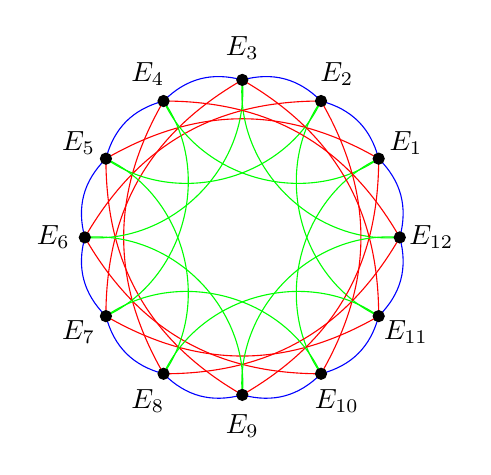
\begin{tikzpicture}
        \begin{scope}
          \def\crater{12}
          \def\jumpa{-8}
          \def\jumpb{9}
          \def\diam{2cm}

          \foreach \i in {1,...,\crater} {
            \draw[blue] (360/\crater*\i : \diam) to[bend right] (360/\crater*\i+360/\crater : \diam);
            \draw[red] (360/\crater*\i : \diam) to[bend right] (360/\crater*\i+\jumpa*360/\crater : \diam);
            \draw[green] (360/\crater*\i : \diam) to[bend right=50] (360/\crater*\i+\jumpb*360/\crater : \diam);
          }
          \foreach \i in {1,...,\crater} {
            \draw[fill] (360/\crater*\i: \diam) circle (2pt) +(360/\crater*\i: 0.4) node{$E_{\i}$};
          }
        \end{scope}
      \end{tikzpicture}
    \end{column}
  \end{columns}
\end{frame}

%% 

{
  \newcommand{\myedge}[3]{
    \draw[#3] (360/\crater*#1 : \diam) to[bend right] (360/\crater*#2 : \diam);
  }
  \begin{frame}{Couveignes / Rostovtsev-Stolbunov / CSIDH key exchange}
    \begin{columns}
      \begin{column}{0.55\textwidth}
        \begin{tikzpicture}
          \begin{scope}
            \def\crater{12}
            \def\jumpa{-8}
            \def\jumpb{9}
            \def\diam{2.5cm}
            
            \foreach \i in {1,...,\crater} {
              \pgfmathparse{int(mod(2^\i,13))}
              \let\exp\pgfmathresult
              \draw[fill] (360/\crater*\i: \diam) circle (2pt);
            }
            \uncover<2,6->{
              % Alice 1
              \myedge{0}{1}{blue}\myedge{1}{5}{red}\myedge{5}{6}{blue}\myedge{6}{3}{green}
            }
            \uncover<3,5>{
              % Bob 1
              \begin{scope}[dashed,thick]
                \myedge{0}{4}{red}\myedge{4}{8}{red}\myedge{8}{5}{green}\myedge{5}{6}{blue}
              \end{scope}
            }
            \uncover<5>{
              % Alice 2
              \myedge{6}{7}{blue}\myedge{7}{11}{red}\myedge{11}{0}{blue}\myedge{0}{9}{green}
            }
            \uncover<6->{
              % Bob 2
              \begin{scope}[dashed,thick]
                \myedge{3}{7}{red}\myedge{7}{11}{red}\myedge{11}{8}{green}\myedge{8}{9}{blue}
              \end{scope}
            }

            \draw (0 : \diam + 0.4cm) node {$E_0$};
            \uncover<2->{\draw (360/\crater*3 : \diam + 0.4cm) node {$E_A$};}
            \uncover<3->{\draw (360/\crater*6 : \diam + 0.4cm) node {$E_B$};}
            \uncover<5->{\draw (360/\crater*9 : \diam + 0.4cm) node {$E_{BA}\uncover<6->{=E_{AB}}$};}
          \end{scope}
        \end{tikzpicture}  
      \end{column}    
      \begin{column}{0.45\textwidth}
        \textbf{Public parameters:}
        \begin{itemize}
        \item A supersingular curve $E_0/\F_p$;
        \item A set of small prime degree isogenies.
        \end{itemize}
        \begin{enumerate}
        \item<2-> \textbf{Alice} takes a \alert{secret} random walk
          \emph{$ϕ_A:E_0\to E_A$} of length \emph{$O(\log p)$};
        \item<3-> \textbf{Bob} does the same;
        \item<4-> They publish \emph{$E_A$} and \emph{$E_B$};
        \item<5-> \textbf{Alice} repeats her secret walk \emph{$ϕ_A$}
          starting from \emph{$E_B$}.
        \item<6-> \textbf{Bob} repeats his secret walk \emph{$ϕ_B$}
          starting from \emph{$E_A$}.
        \end{enumerate}
      \end{column}
    \end{columns}
  \end{frame}
}

%%

\begin{frame}[plain]
  \centering
  \begin{tikzpicture}[remember picture,overlay]
    \begin{scope}[xscale=1.7,yshift=-15,opacity=0.8]
      \def\crater{12}
      \def\jumpa{-8}
      \def\jumpb{9}
      \def\diam{5cm}

      \foreach \i in {1,...,\crater} {
        \draw[blue] (360/\crater*\i : \diam) to[bend right] (360/\crater*\i+360/\crater : \diam);
        \draw[red] (360/\crater*\i : \diam) to[bend right] (360/\crater*\i+\jumpa*360/\crater : \diam);
        \draw[green] (360/\crater*\i : \diam) to[bend right=50] (360/\crater*\i+\jumpb*360/\crater : \diam);
      }
    \end{scope}
    
    \draw (0,0.5) node{\Huge\bf Thank you};
    \draw (0,-0.6) node{\large\url{https://defeo.lu/}};
    \draw (0,-1.3) node{\large\includegraphics[height=0.9em]{mastodon.png}~\href{https://twitter.com/luca_defeo}{@luca\_defeo@ioc.exchange}};
    \draw (0,-1.9) node{\large\includegraphics[height=0.9em]{twitter.png}~\href{https://twitter.com/luca_defeo}{@luca\_defeo}};
  \end{tikzpicture}
\end{frame}

%%

\end{document}


% LocalWords:  Isogeny abelian isogenies hyperelliptic supersingular Frobenius
% LocalWords:  isogenous
